\begin{center}
  {\LARGE\bfseries Dr. Debiprasad Duari Takes STCET Audience on a Journey to Astronomy's New Frontiers\par}
  \vspace{0.45em}
  {\large\bfseries\color{IEEEblue}
  Interactive seminar connects cosmic discovery, space technology and India's expanding role in exploration.\par}
  \vspace{0.5em}
  {\small\itshape By the Editorial Desk}
\end{center}

\begin{tcolorbox}[
  colback=SoftBlue,
  colframe=IEEEblue!75!black,
  boxrule=0.6pt,
  arc=0mm,
  left=3mm,right=3mm,top=2mm,bottom=2mm
]
  \small\RaggedRight
  \textbf{At a glance:} The interactive seminar, titled ``Astronomy: Frontiers of S\&T,'' featured astrophysicist and science communicator Dr. Debiprasad Duari. It was co-organised at STCET by the IEEE CIS \& IES Student Chapter, the IEEE WIE Student Branch Affinity Group, and the Institution's Innovation Council (IIC).
\end{tcolorbox}

\begin{center}
  \setlength{\tabcolsep}{2pt}
  \begin{tabular}{@{}cc@{}}
    \includegraphics[width=0.4\textwidth]{assets/images/ast-3.jpeg} &
    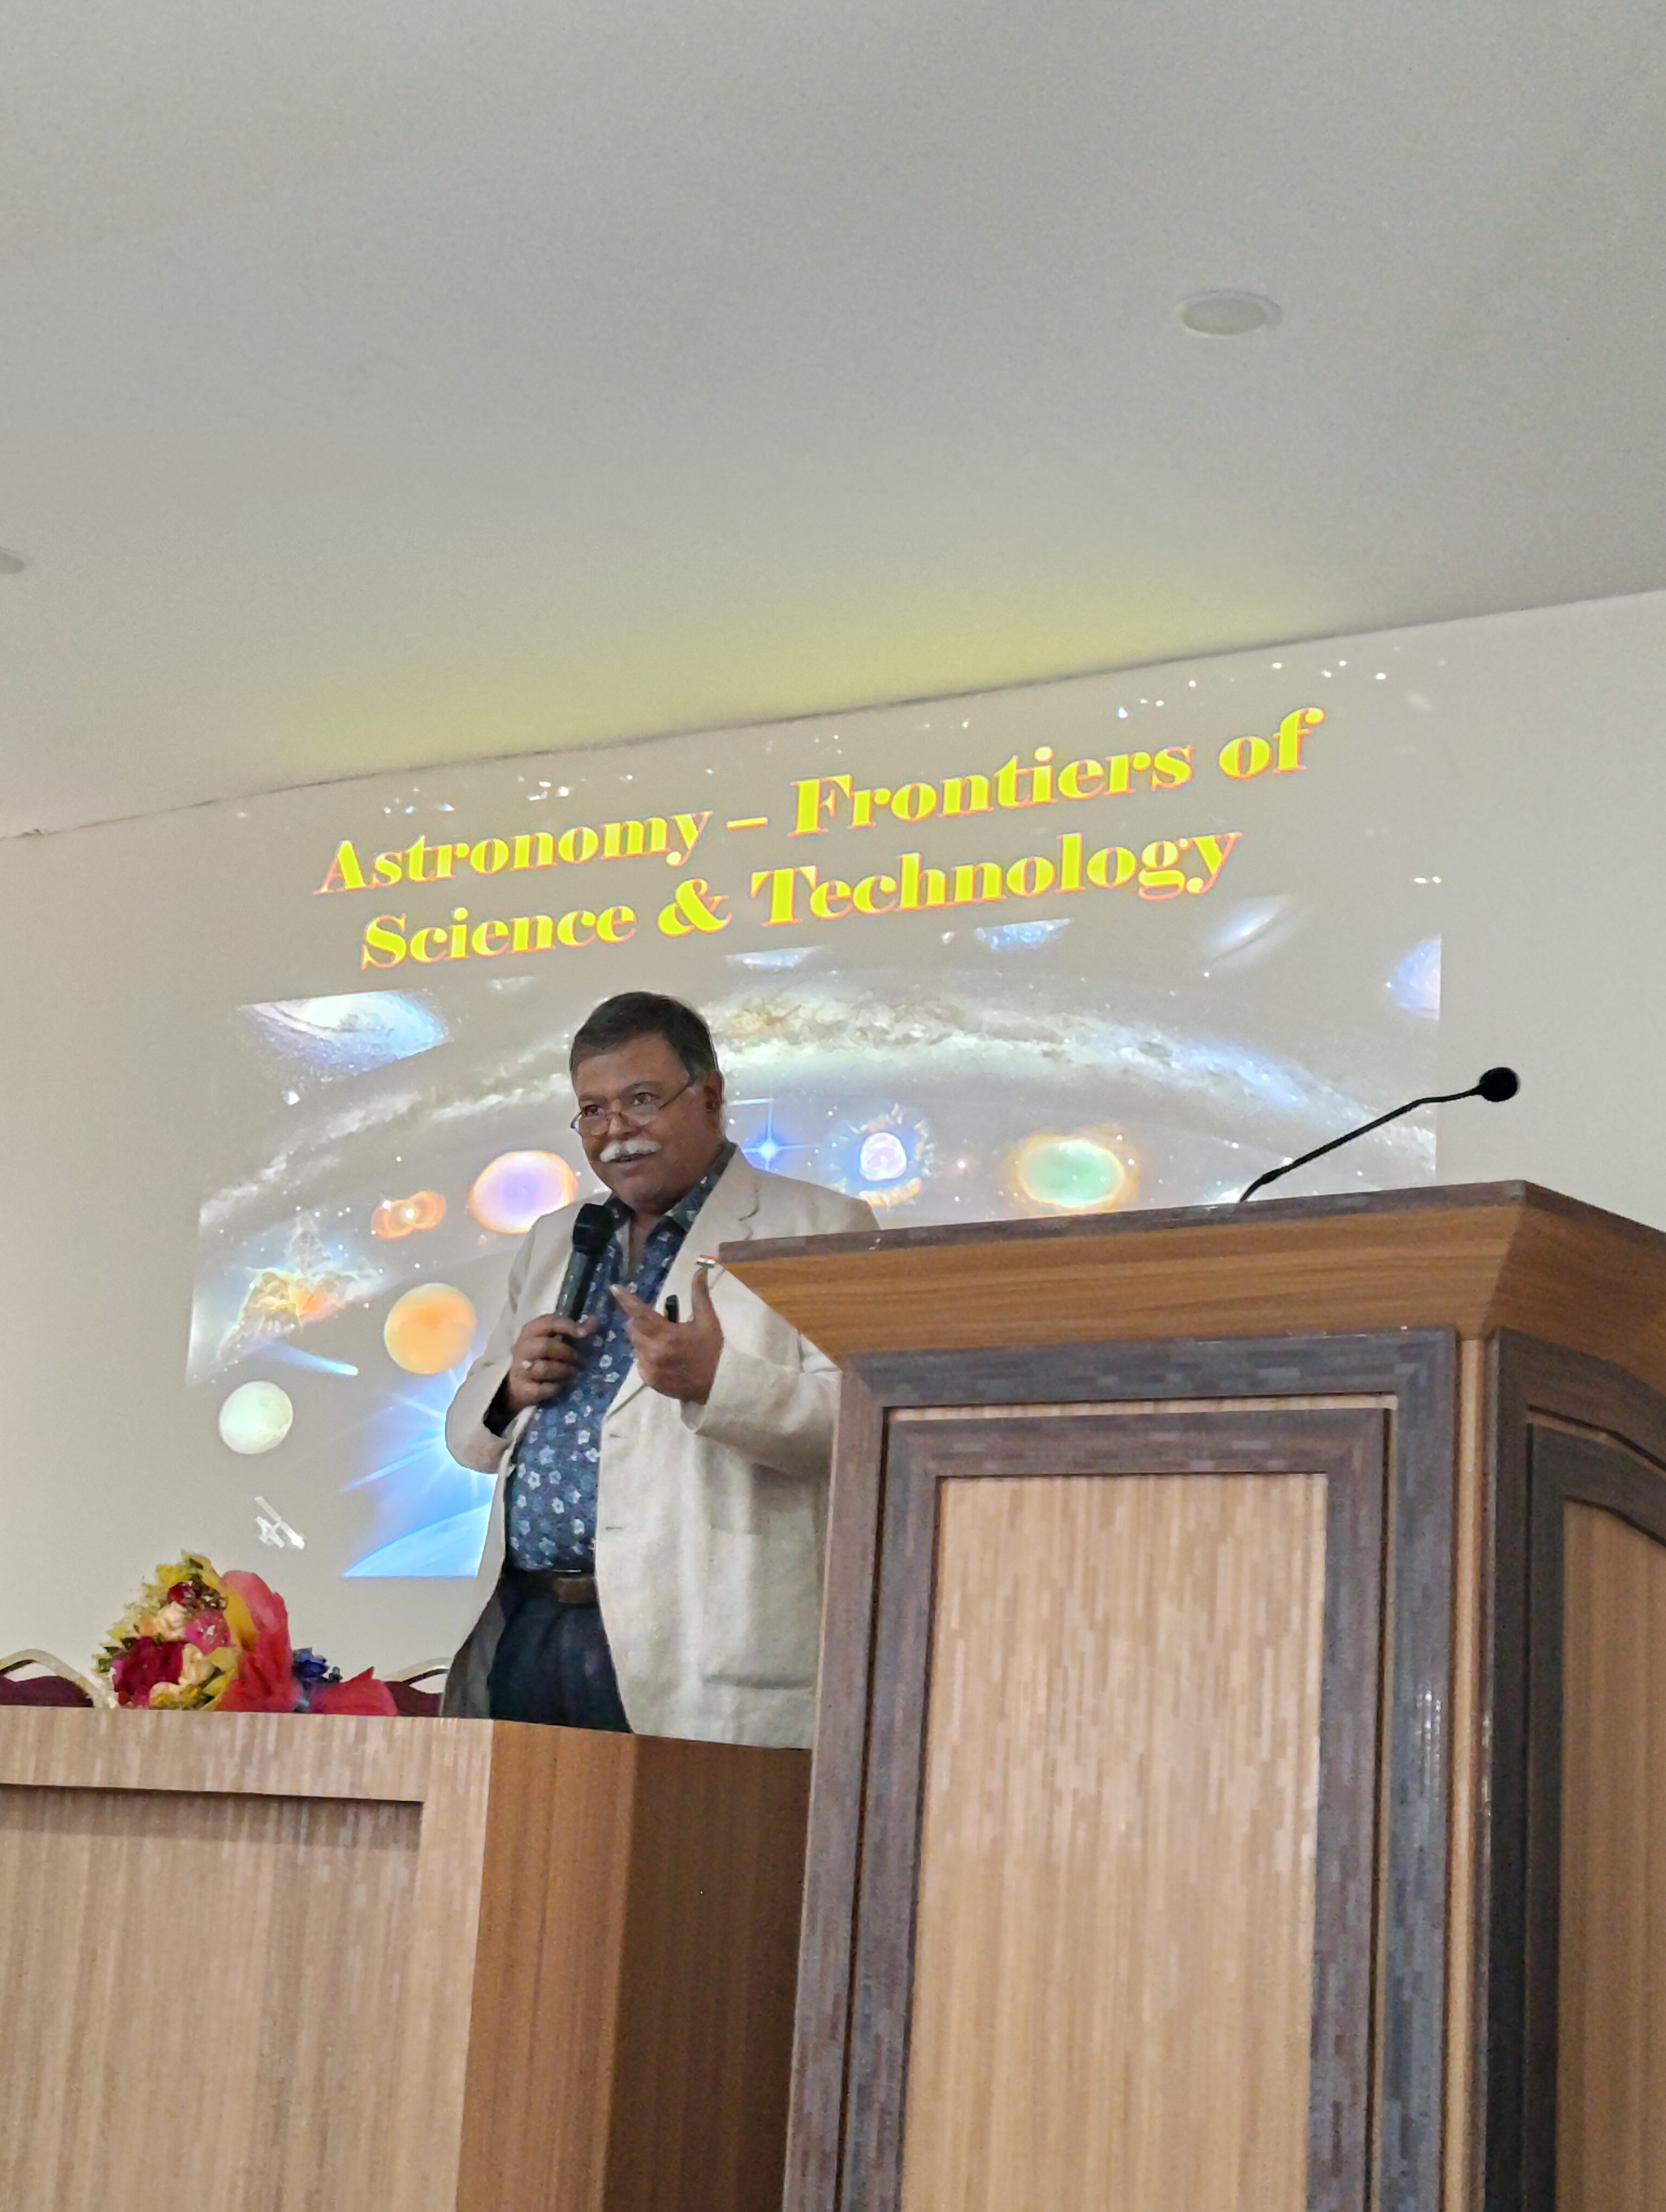
\includegraphics[width=0.4\textwidth]{assets/images/ast-4.jpeg}
  \end{tabular}
\end{center}

{\small
\noindent
\textbf{Kolkata, February 13, 2026---}The scale of the universe met the curiosity of a young engineering audience at St. Thomas' College of Engineering \& Technology (STCET), where renowned astrophysicist Dr. Debiprasad Duari delivered an engaging seminar on ``Astronomy: Frontiers of S\&T.'' Co-organised by the IEEE Computational Intelligence Society (CIS) \& Industrial Electronics Society (IES) Student Chapter, the IEEE Women in Engineering (WIE) Student Branch Affinity Group, and the Institution's Innovation Council (IIC) at STCET, the programme brought students, faculty members and young researchers together for a wide-ranging exploration of modern astronomy and space science.

\medskip
\noindent
Dr. Duari presented astronomy not as a distant catalogue of stars and planets, but as a rapidly advancing field shaped by engineering, computation and international scientific collaboration. His address moved from the familiar architecture of the solar system to the formation of stars and the immense physical processes that govern cosmic phenomena. Complex ideas were communicated in an accessible manner, allowing participants from different academic backgrounds to follow the scientific story without losing sight of its scale or significance.

\medskip
\noindent
A central theme of the session was the convergence of science and technology. Astronomers may begin with fundamental questions---how stars are born, how planetary systems evolve, what lies beyond visible light, and how the universe changes over time---but answering them depends on precision instruments and sophisticated engineering. Telescopes, detectors, satellites, communication links, signal-processing systems, control electronics and large-scale computation have become essential tools for turning faint radiation from space into reliable scientific knowledge.

\medskip
\noindent
The seminar highlighted how each technological advance opens a new observational window. More sensitive detectors reveal objects that earlier instruments could not distinguish; space-based observatories avoid many limitations imposed by Earth's atmosphere; improved electronics allow weak signals to be measured with greater accuracy; and computational methods help researchers process enormous datasets, compare models and identify patterns hidden within noise. The result is a field in which discoveries are often made at the intersection of physics, electronics, communication engineering, data science and intelligent systems.

\medskip
\noindent
Dr. Duari also placed contemporary space exploration within a broader historical transition. The 21st century, he observed, is poised to become a defining period for exploration beyond Earth. Space activity is no longer limited to a small number of national agencies or isolated scientific missions. Universities, research laboratories, start-ups and private companies increasingly contribute instruments, software, small satellites, launch technologies and data-driven services.

\medskip
\noindent
India's growing achievements in space science and technology formed an important part of the discussion. The country's expanding capabilities in launch systems, planetary missions, satellite applications and scientific observation demonstrate how long-term investment in engineering can support both fundamental research and practical national needs. For students, this development creates a widening range of possibilities in spacecraft electronics, remote sensing, communication, navigation, embedded systems, robotics, materials, control engineering and scientific computing.

\medskip
\noindent
The session gained particular energy when the formal lecture opened into an interactive exchange. Students responded with enthusiasm, seeking to connect the ideas presented on stage with questions about the origin and evolution of celestial objects, the limits of present-day observation, future missions and the skills required to enter space-related research. Faculty members and young researchers added questions that linked astronomy with engineering design, computation and interdisciplinary collaboration.

\begin{center}
  \setlength{\tabcolsep}{3pt}
  \begin{tabular}{@{}cc@{}}
    \includegraphics[height=0.35 \textheight]{assets/images/ast-2.jpeg} &
    \includegraphics[height=0.35\textheight]{assets/images/ast-5.jpeg}
  \end{tabular}
\end{center}

\medskip
\noindent
Rather than treating the question-and-answer segment as an appendix to the lecture, Dr. Duari used it to reinforce the method of science itself. Questions that do not yet have complete answers are not failures, the discussion suggested, but starting points for observation, modelling and experiment. The exchange encouraged participants to distinguish established evidence from speculation and to see curiosity as a disciplined habit that must be supported by mathematics, measurement and critical reasoning.

\medskip
\noindent
The audience engagement also demonstrated the value of direct interaction with an experienced science communicator. Astronomy often captures attention through striking images and extraordinary distances, but its deeper educational value lies in the way it unites multiple branches of knowledge. A discussion about a star can involve nuclear physics, spectroscopy, electronics, statistics and computer simulation; a planetary mission can require orbital mechanics, sensors, antennas, autonomous control and reliable software. For engineering students, the field offers a vivid example of why complex problems rarely remain confined to one discipline.

\medskip
\noindent
The participation of the organising bodies reflected that same interdisciplinary outlook. The IEEE CIS \& IES Student Chapter brought perspectives from intelligent computation and industrial electronics, while the IEEE WIE Student Branch Affinity Group reinforced the importance of inclusive participation in science and engineering. The IIC's involvement placed the seminar within the institution's wider effort to promote innovation, research awareness and the translation of ideas into technological possibilities.

\medskip
\noindent
High-calibre scientific talks of this kind can have an impact beyond the duration of a single event. They expose students to research questions that may not appear in a conventional syllabus, introduce possible career pathways and make advanced science feel more approachable. A student initially drawn by the spectacle of space may leave thinking seriously about instrumentation, antenna design, image processing, artificial intelligence, satellite communication or astrophysical research.

\medskip
\noindent
The programme was also a reminder that scientific ambition depends on sustained learning. Space research requires strong foundations, patient experimentation and the willingness to work across disciplinary boundaries. Dr. Duari's accessible presentation encouraged participants to dream boldly while recognising the preparation needed to convert fascination into meaningful study and innovation.

\medskip
\noindent
By the close of the seminar, ``Astronomy: Frontiers of S\&T'' had succeeded in bringing the universe closer to the campus. Its strongest takeaway was not a single fact about a planet or star, but a larger message: cosmic mysteries become answerable when human curiosity is joined with rigorous science, imaginative engineering and technology capable of extending our senses far beyond Earth.

\begin{center}
  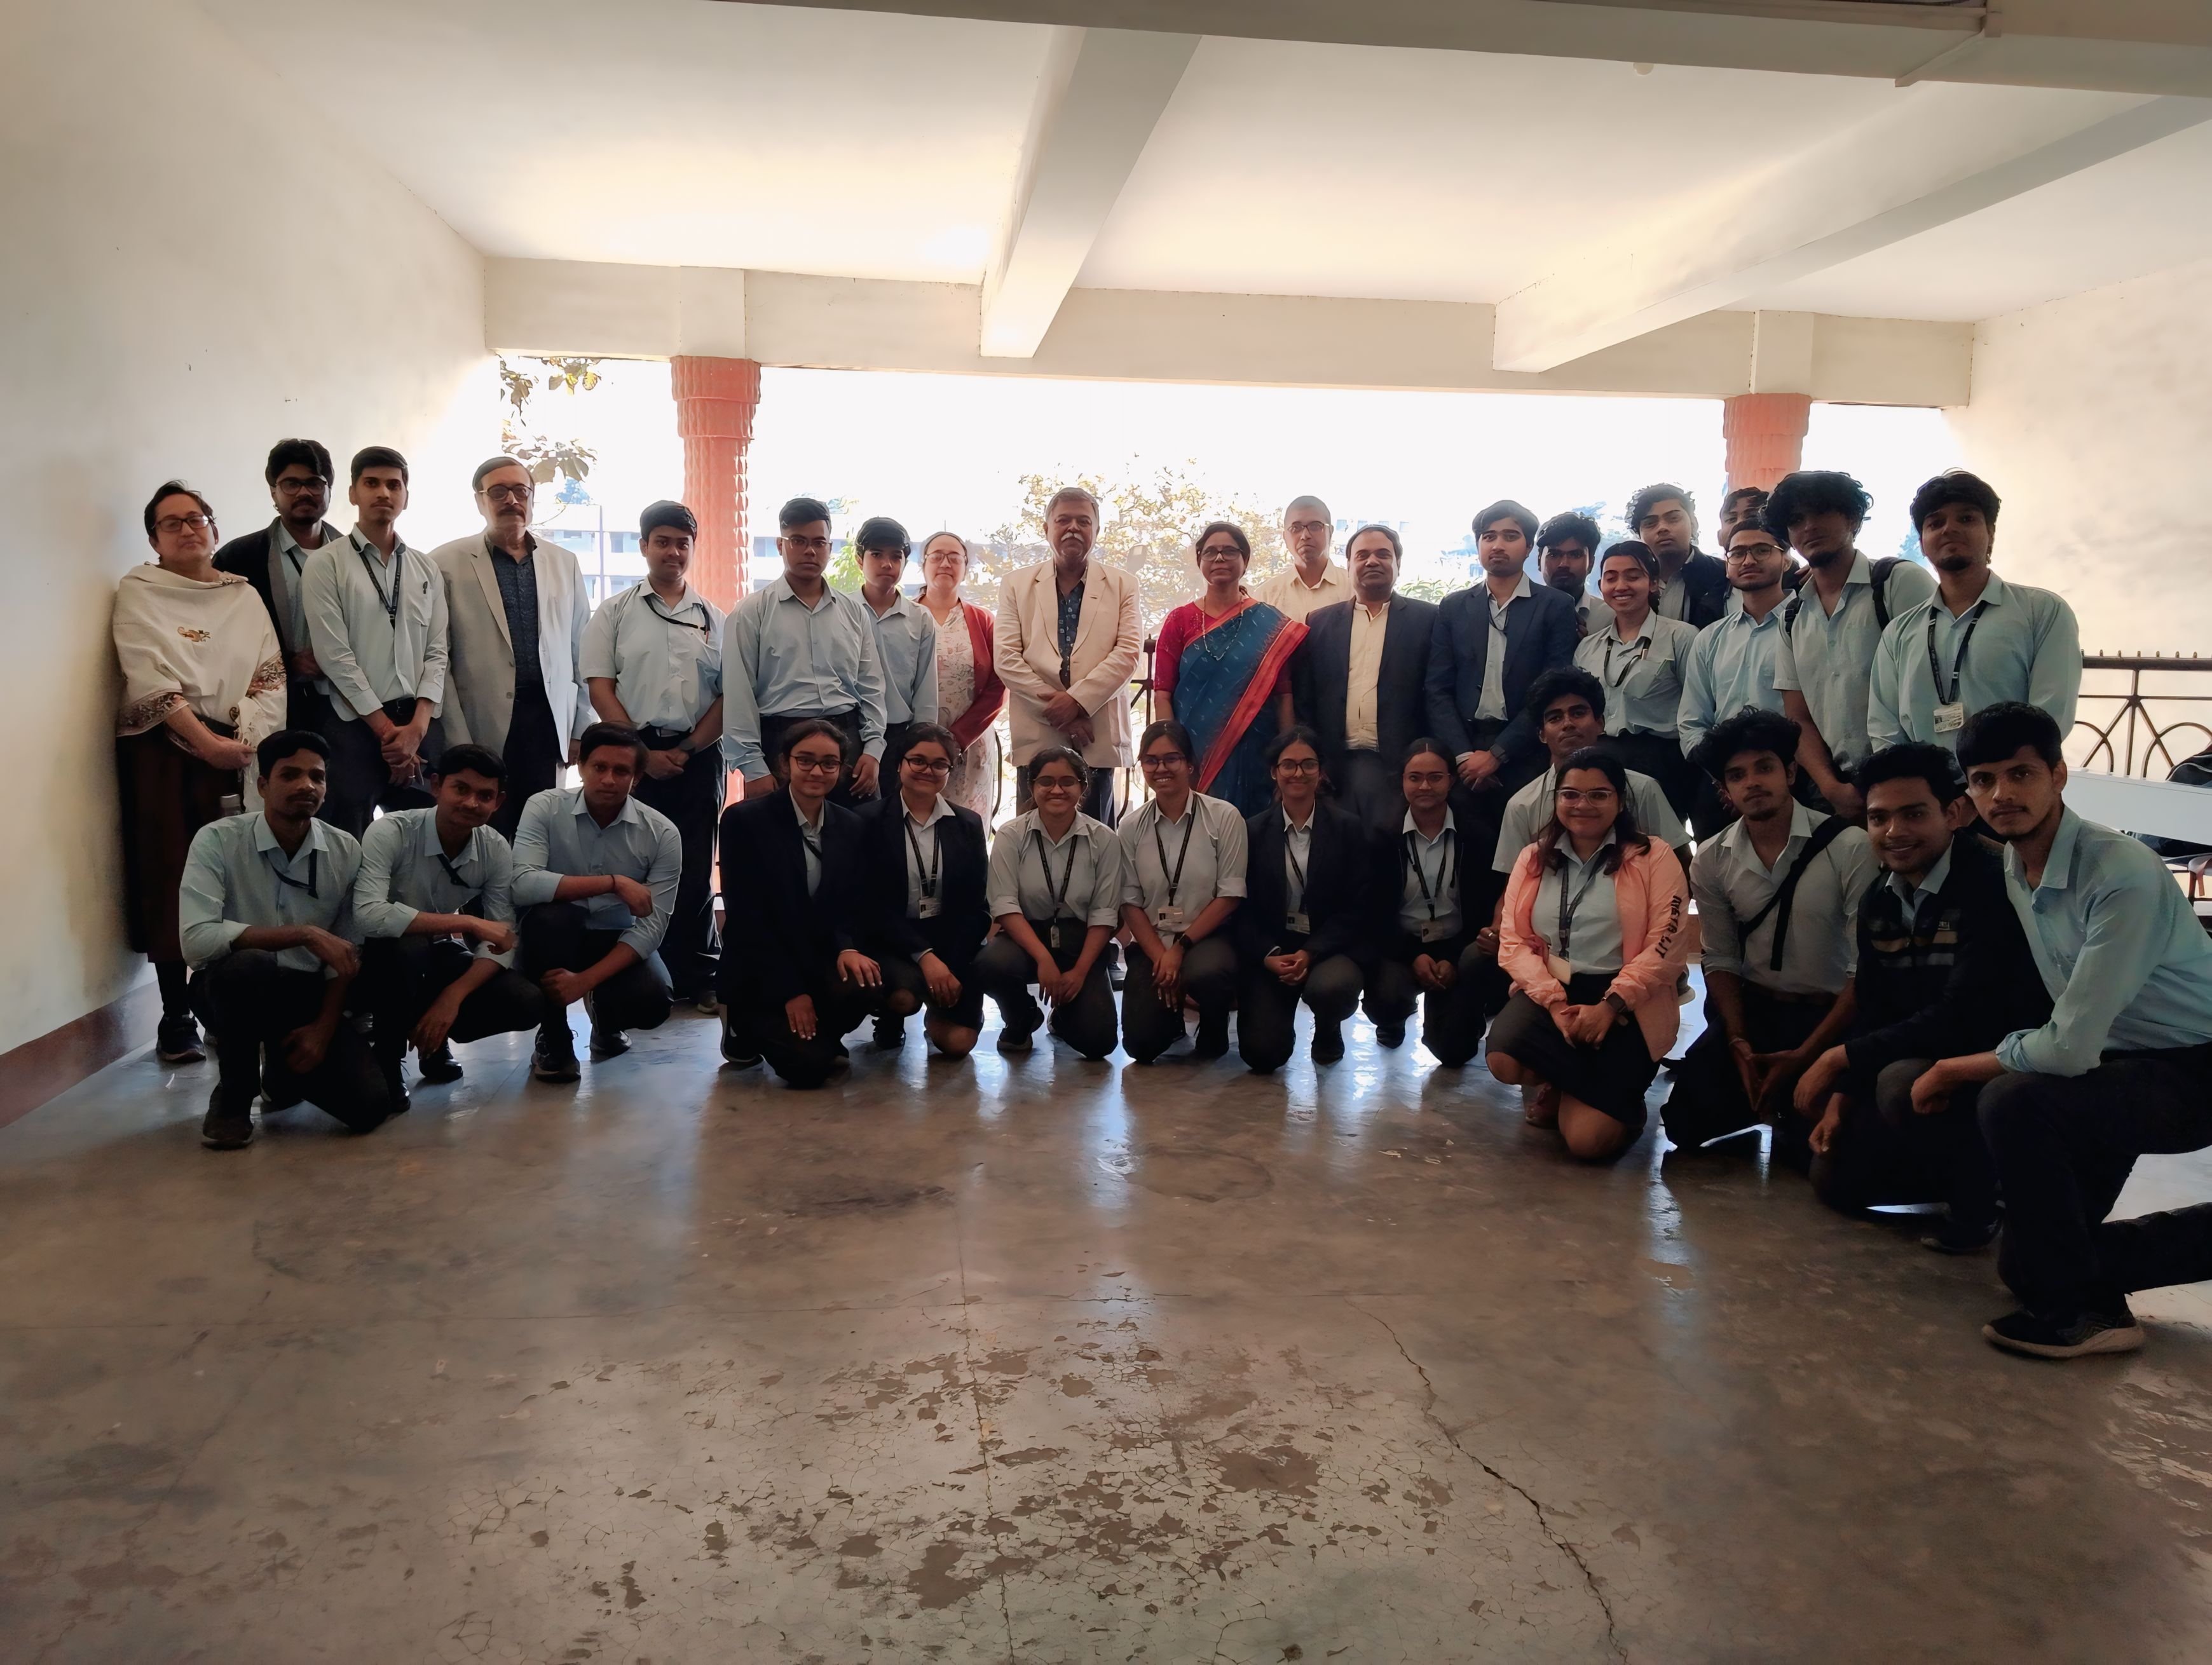
\includegraphics[width=0.8\textwidth]{assets/images/ast-1.jpeg}
\end{center}
\par}

\vfill
\noindent
{\footnotesize\sloppy\textit{Source note: The event theme, organisers and interactive format are based on the programme brief. Key lecture themes are supported by a published account of Dr. Duari's STCET address, which described his discussion of the solar system, star formation, cosmic phenomena, India's space achievements and the future of exploration.}\par}